% Options for packages loaded elsewhere
\PassOptionsToPackage{unicode}{hyperref}
\PassOptionsToPackage{hyphens}{url}
%
\documentclass[
  ignorenonframetext,
]{beamer}
\usepackage{pgfpages}
\setbeamertemplate{caption}[numbered]
\setbeamertemplate{caption label separator}{: }
\setbeamercolor{caption name}{fg=normal text.fg}
\beamertemplatenavigationsymbolsempty
% Prevent slide breaks in the middle of a paragraph
\widowpenalties 1 10000
\raggedbottom
\setbeamertemplate{part page}{
  \centering
  \begin{beamercolorbox}[sep=16pt,center]{part title}
    \usebeamerfont{part title}\insertpart\par
  \end{beamercolorbox}
}
\setbeamertemplate{section page}{
  \centering
  \begin{beamercolorbox}[sep=12pt,center]{part title}
    \usebeamerfont{section title}\insertsection\par
  \end{beamercolorbox}
}
\setbeamertemplate{subsection page}{
  \centering
  \begin{beamercolorbox}[sep=8pt,center]{part title}
    \usebeamerfont{subsection title}\insertsubsection\par
  \end{beamercolorbox}
}
\AtBeginPart{
  \frame{\partpage}
}
\AtBeginSection{
  \ifbibliography
  \else
    \frame{\sectionpage}
  \fi
}
\AtBeginSubsection{
  \frame{\subsectionpage}
}

\usepackage{amsmath,amssymb}
\usepackage{iftex}
\ifPDFTeX
  \usepackage[T1]{fontenc}
  \usepackage[utf8]{inputenc}
  \usepackage{textcomp} % provide euro and other symbols
\else % if luatex or xetex
  \usepackage{unicode-math}
  \defaultfontfeatures{Scale=MatchLowercase}
  \defaultfontfeatures[\rmfamily]{Ligatures=TeX,Scale=1}
\fi
\usepackage{lmodern}
\ifPDFTeX\else  
    % xetex/luatex font selection
\fi
% Use upquote if available, for straight quotes in verbatim environments
\IfFileExists{upquote.sty}{\usepackage{upquote}}{}
\IfFileExists{microtype.sty}{% use microtype if available
  \usepackage[]{microtype}
  \UseMicrotypeSet[protrusion]{basicmath} % disable protrusion for tt fonts
}{}
\makeatletter
\@ifundefined{KOMAClassName}{% if non-KOMA class
  \IfFileExists{parskip.sty}{%
    \usepackage{parskip}
  }{% else
    \setlength{\parindent}{0pt}
    \setlength{\parskip}{6pt plus 2pt minus 1pt}}
}{% if KOMA class
  \KOMAoptions{parskip=half}}
\makeatother
\usepackage{xcolor}
\newif\ifbibliography
\setlength{\emergencystretch}{3em} % prevent overfull lines
\setcounter{secnumdepth}{-\maxdimen} % remove section numbering


\providecommand{\tightlist}{%
  \setlength{\itemsep}{0pt}\setlength{\parskip}{0pt}}\usepackage{longtable,booktabs,array}
\usepackage{calc} % for calculating minipage widths
\usepackage{caption}
% Make caption package work with longtable
\makeatletter
\def\fnum@table{\tablename~\thetable}
\makeatother
\usepackage{graphicx}
\makeatletter
\def\maxwidth{\ifdim\Gin@nat@width>\linewidth\linewidth\else\Gin@nat@width\fi}
\def\maxheight{\ifdim\Gin@nat@height>\textheight\textheight\else\Gin@nat@height\fi}
\makeatother
% Scale images if necessary, so that they will not overflow the page
% margins by default, and it is still possible to overwrite the defaults
% using explicit options in \includegraphics[width, height, ...]{}
\setkeys{Gin}{width=\maxwidth,height=\maxheight,keepaspectratio}
% Set default figure placement to htbp
\makeatletter
\def\fps@figure{htbp}
\makeatother

\usepackage{booktabs}
\usepackage{longtable}
\usepackage{array}
\usepackage{multirow}
\usepackage{wrapfig}
\usepackage{float}
\usepackage{colortbl}
\usepackage{pdflscape}
\usepackage{tabu}
\usepackage{threeparttable}
\usepackage{threeparttablex}
\usepackage[normalem]{ulem}
\usepackage{makecell}
\usepackage{xcolor}
\makeatletter
\makeatother
\makeatletter
\makeatother
\makeatletter
\@ifpackageloaded{caption}{}{\usepackage{caption}}
\AtBeginDocument{%
\ifdefined\contentsname
  \renewcommand*\contentsname{Table of contents}
\else
  \newcommand\contentsname{Table of contents}
\fi
\ifdefined\listfigurename
  \renewcommand*\listfigurename{List of Figures}
\else
  \newcommand\listfigurename{List of Figures}
\fi
\ifdefined\listtablename
  \renewcommand*\listtablename{List of Tables}
\else
  \newcommand\listtablename{List of Tables}
\fi
\ifdefined\figurename
  \renewcommand*\figurename{Figure}
\else
  \newcommand\figurename{Figure}
\fi
\ifdefined\tablename
  \renewcommand*\tablename{Table}
\else
  \newcommand\tablename{Table}
\fi
}
\@ifpackageloaded{float}{}{\usepackage{float}}
\floatstyle{ruled}
\@ifundefined{c@chapter}{\newfloat{codelisting}{h}{lop}}{\newfloat{codelisting}{h}{lop}[chapter]}
\floatname{codelisting}{Listing}
\newcommand*\listoflistings{\listof{codelisting}{List of Listings}}
\makeatother
\makeatletter
\@ifpackageloaded{caption}{}{\usepackage{caption}}
\@ifpackageloaded{subcaption}{}{\usepackage{subcaption}}
\makeatother
\makeatletter
\@ifpackageloaded{tcolorbox}{}{\usepackage[skins,breakable]{tcolorbox}}
\makeatother
\makeatletter
\@ifundefined{shadecolor}{\definecolor{shadecolor}{rgb}{.97, .97, .97}}
\makeatother
\makeatletter
\makeatother
\makeatletter
\makeatother
\ifLuaTeX
  \usepackage{selnolig}  % disable illegal ligatures
\fi
\IfFileExists{bookmark.sty}{\usepackage{bookmark}}{\usepackage{hyperref}}
\IfFileExists{xurl.sty}{\usepackage{xurl}}{} % add URL line breaks if available
\urlstyle{same} % disable monospaced font for URLs
\hypersetup{
  pdftitle={Multiple Regression},
  hidelinks,
  pdfcreator={LaTeX via pandoc}}

\title{Multiple Regression}
\author{}
\date{}

\begin{document}
\frame{\titlepage}
\ifdefined\Shaded\renewenvironment{Shaded}{\begin{tcolorbox}[interior hidden, borderline west={3pt}{0pt}{shadecolor}, sharp corners, enhanced, breakable, frame hidden, boxrule=0pt]}{\end{tcolorbox}}\fi

\begin{frame}{}
\protect\hypertarget{section}{}
\begin{longtable}[]{@{}rrr@{}}
\toprule\noalign{}
biking & smoking & heart\_disease \\
\midrule\noalign{}
\endhead
30.801246 & 10.896608 & 11.769423 \\
65.129215 & 2.219563 & 2.854081 \\
1.959664 & 17.588331 & 17.177803 \\
44.800196 & 2.802559 & 6.816647 \\
69.428454 & 15.974505 & 4.062223 \\
54.403626 & 29.333175 & 9.550046 \\
49.056162 & 9.060846 & 7.624507 \\
4.784604 & 12.835021 & 15.854654 \\
65.730788 & 11.991297 & 3.067462 \\
35.257449 & 23.277683 & 12.098484 \\
51.825567 & 14.435118 & 6.430248 \\
52.936197 & 25.074869 & 8.608272 \\
48.767479 & 11.023271 & 6.722524 \\
26.166801 & 6.645749 & 10.597807 \\
10.553075 & 5.990506 & 14.079478 \\
\bottomrule\noalign{}
\end{longtable}
\end{frame}

\begin{frame}{Multiple Regression Model}
\protect\hypertarget{multiple-regression-model}{}
\[
\text{heart_disease} = \beta_0 + \beta_1\cdot \text{biking} + \beta_2\cdot \text{smoking} + \epsilon
\] - \(\epsilon \sim N(0, \sigma^2)\)
\end{frame}

\begin{frame}{Graphing the solution}
\protect\hypertarget{graphing-the-solution}{}
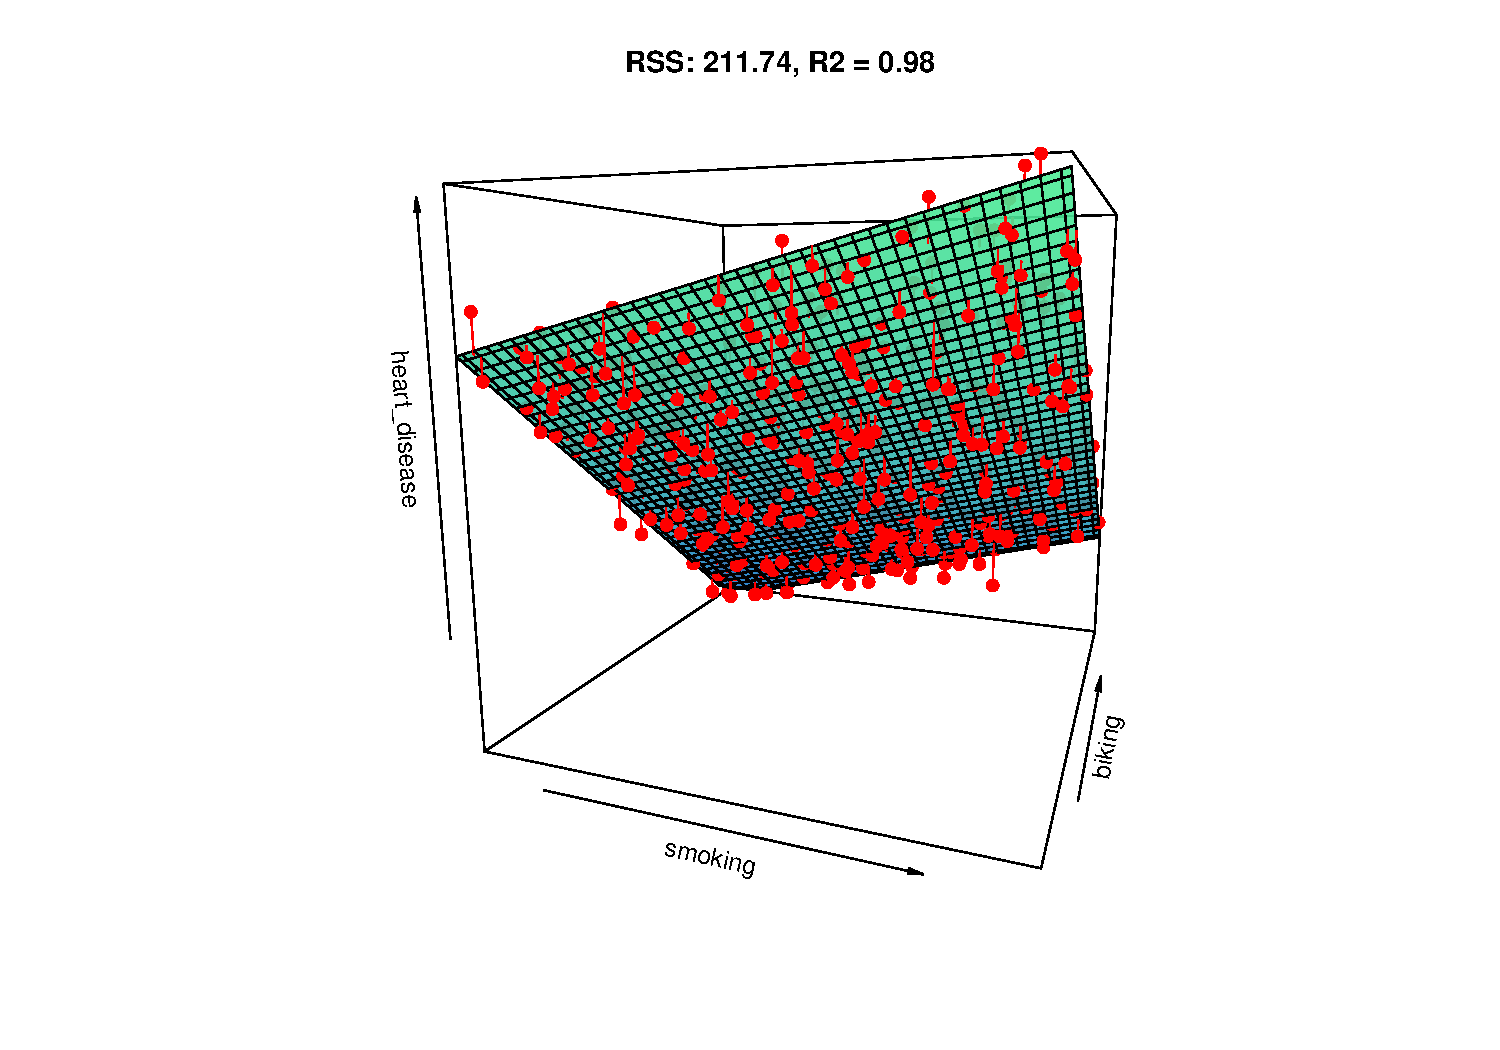
\includegraphics{2_1_files/figure-beamer/unnamed-chunk-4-1.pdf}

\begin{itemize}
\tightlist
\item
  heart\_disease = 14.984658 + -0.2001331 \(\cdot\) biking + 0.1783339
  \(\cdot\) smoking
\end{itemize}
\end{frame}

\begin{frame}{Model Definition}
\protect\hypertarget{model-definition}{}
\end{frame}

\begin{frame}{}
\protect\hypertarget{section-1}{}
\begin{center}
\Huge Parameters Estimation
\end{center}
\end{frame}

\begin{frame}{}
\protect\hypertarget{section-2}{}
\[
\hat{\beta} = (X'X)^{-1}X'y
\]
\end{frame}

\begin{frame}{}
\protect\hypertarget{section-3}{}
\begin{table}[!h]
\centering
\begin{tabular}{lr}
\toprule
\cellcolor{gray!6}{Observations} & \cellcolor{gray!6}{498}\\
Dependent variable & heart\_disease\\
\cellcolor{gray!6}{Type} & \cellcolor{gray!6}{OLS linear regression}\\
\bottomrule
\end{tabular}
\end{table} \begin{table}[!h]
\centering
\begin{tabular}{lr}
\toprule
\cellcolor{gray!6}{F(2,495)} & \cellcolor{gray!6}{11895.241}\\
R² & 0.980\\
\cellcolor{gray!6}{Adj. R²} & \cellcolor{gray!6}{0.980}\\
\bottomrule
\end{tabular}
\end{table} \begin{table}[!h]
\centering
\begin{threeparttable}
\begin{tabular}{lrrrr}
\toprule
  & Est. & S.E. & t val. & p\\
\midrule
\cellcolor{gray!6}{(Intercept)} & \cellcolor{gray!6}{14.985} & \cellcolor{gray!6}{0.080} & \cellcolor{gray!6}{186.988} & \cellcolor{gray!6}{0.000}\\
biking & -0.200 & 0.001 & -146.525 & 0.000\\
\cellcolor{gray!6}{smoking} & \cellcolor{gray!6}{0.178} & \cellcolor{gray!6}{0.004} & \cellcolor{gray!6}{50.387} & \cellcolor{gray!6}{0.000}\\
\bottomrule
\end{tabular}
\begin{tablenotes}
\item Standard errors: OLS
\end{tablenotes}
\end{threeparttable}
\end{table}
\end{frame}

\begin{frame}{}
\protect\hypertarget{section-4}{}
\begin{center}
\Huge Goodness of Fit
\end{center}
\end{frame}

\begin{frame}{}
\protect\hypertarget{section-5}{}
\begin{center}
\Huge Colinearity
\end{center}
\end{frame}

\begin{frame}{}
\protect\hypertarget{section-6}{}
\begin{table}
\centering\begingroup\fontsize{8}{10}\selectfont

\begin{tabular}[t]{r|r|r|r|r|r|r|r|r}
\hline
Age & Weight & HtShoes & Ht & Seated & Arm & Thigh & Leg & hipcenter\\
\hline
46 & 180 & 187.2 & 184.9 & 95.2 & 36.1 & 45.3 & 41.3 & -206.300\\
\hline
31 & 175 & 167.5 & 165.5 & 83.8 & 32.9 & 36.5 & 35.9 & -178.210\\
\hline
23 & 100 & 153.6 & 152.2 & 82.9 & 26.0 & 36.6 & 31.0 & -71.673\\
\hline
19 & 185 & 190.3 & 187.4 & 97.3 & 37.4 & 44.1 & 41.0 & -257.720\\
\hline
23 & 159 & 178.0 & 174.1 & 93.9 & 29.5 & 40.1 & 36.9 & -173.230\\
\hline
47 & 170 & 178.7 & 177.0 & 92.4 & 36.0 & 43.2 & 37.4 & -185.150\\
\hline
30 & 137 & 165.7 & 164.6 & 87.7 & 32.5 & 35.6 & 36.2 & -164.750\\
\hline
28 & 192 & 185.3 & 182.7 & 96.9 & 35.8 & 39.9 & 43.1 & -270.920\\
\hline
23 & 150 & 167.6 & 165.0 & 91.4 & 29.4 & 35.5 & 33.4 & -151.780\\
\hline
29 & 120 & 161.2 & 158.7 & 85.2 & 26.6 & 31.0 & 32.8 & -113.880\\
\hline
47 & 143 & 171.9 & 169.1 & 87.8 & 32.9 & 39.2 & 36.9 & -196.150\\
\hline
41 & 107 & 155.7 & 152.5 & 82.9 & 29.6 & 32.7 & 31.1 & -125.550\\
\hline
51 & 227 & 179.8 & 177.2 & 91.7 & 31.1 & 41.4 & 40.2 & -203.610\\
\hline
30 & 147 & 164.9 & 162.7 & 88.0 & 27.7 & 33.6 & 33.8 & -163.220\\
\hline
22 & 178 & 177.2 & 176.4 & 94.1 & 31.1 & 41.0 & 36.6 & -204.110\\
\hline
67 & 166 & 177.1 & 175.3 & 89.4 & 36.7 & 40.1 & 39.2 & -186.800\\
\hline
25 & 153 & 173.4 & 171.2 & 85.0 & 33.1 & 45.2 & 38.4 & -228.350\\
\hline
65 & 113 & 162.6 & 158.7 & 85.2 & 31.1 & 35.7 & 32.5 & -103.850\\
\hline
22 & 142 & 167.3 & 164.6 & 90.4 & 29.5 & 36.5 & 34.0 & -105.690\\
\hline
21 & 130 & 172.5 & 170.5 & 89.7 & 29.9 & 35.8 & 35.6 & -137.360\\
\hline
20 & 145 & 168.4 & 166.3 & 87.9 & 30.3 & 34.6 & 38.5 & -133.080\\
\hline
33 & 293 & 201.2 & 198.4 & 101.6 & 39.6 & 44.2 & 43.1 & -279.150\\
\hline
24 & 180 & 187.6 & 185.3 & 92.6 & 34.9 & 39.9 & 41.8 & -185.870\\
\hline
39 & 117 & 152.8 & 150.2 & 79.4 & 28.9 & 34.8 & 30.2 & -30.950\\
\hline
58 & 150 & 169.2 & 166.4 & 86.2 & 33.0 & 37.9 & 35.7 & -196.550\\
\hline
22 & 171 & 184.1 & 181.6 & 95.4 & 33.7 & 41.8 & 39.2 & -205.610\\
\hline
21 & 125 & 165.8 & 163.4 & 85.0 & 31.0 & 36.4 & 35.3 & -94.502\\
\hline
23 & 160 & 166.4 & 164.3 & 86.2 & 29.1 & 36.6 & 31.6 & -125.840\\
\hline
21 & 157 & 177.0 & 175.5 & 91.4 & 34.4 & 41.6 & 36.4 & -222.500\\
\hline
40 & 115 & 153.8 & 151.6 & 80.3 & 27.5 & 37.6 & 31.7 & -102.200\\
\hline
59 & 168 & 155.2 & 153.0 & 84.4 & 34.1 & 35.6 & 34.6 & -47.520\\
\hline
47 & 175 & 176.6 & 175.8 & 90.9 & 34.5 & 45.5 & 37.4 & -183.550\\
\hline
72 & 186 & 177.7 & 175.0 & 90.1 & 38.3 & 39.7 & 37.7 & -118.050\\
\hline
34 & 115 & 155.2 & 152.2 & 82.0 & 28.9 & 32.9 & 32.6 & -148.670\\
\hline
19 & 150 & 172.2 & 169.9 & 89.4 & 34.0 & 39.7 & 38.1 & -268.320\\
\hline
41 & 121 & 166.3 & 164.1 & 86.5 & 31.5 & 45.1 & 33.8 & -117.000\\
\hline
21 & 154 & 172.0 & 170.4 & 90.0 & 29.5 & 36.8 & 37.5 & -201.510\\
\hline
56 & 158 & 173.8 & 171.5 & 90.0 & 36.1 & 39.2 & 35.5 & -176.450\\
\hline
\end{tabular}
\endgroup{}
\end{table}
\end{frame}

\begin{frame}{}
\protect\hypertarget{section-7}{}
\begin{table}[!h]
\centering
\begin{tabular}{lr}
\toprule
\cellcolor{gray!6}{F(8,29)} & \cellcolor{gray!6}{7.94}\\
R² & 0.69\\
\cellcolor{gray!6}{Adj. R²} & \cellcolor{gray!6}{0.60}\\
\bottomrule
\end{tabular}
\end{table} \begin{table}[!h]
\centering
\begin{threeparttable}
\begin{tabular}{lrrrr}
\toprule
  & Est. & S.E. & t val. & p\\
\midrule
\cellcolor{gray!6}{(Intercept)} & \cellcolor{gray!6}{436.43} & \cellcolor{gray!6}{166.57} & \cellcolor{gray!6}{2.62} & \cellcolor{gray!6}{0.01}\\
Age & 0.78 & 0.57 & 1.36 & 0.18\\
\cellcolor{gray!6}{Weight} & \cellcolor{gray!6}{0.03} & \cellcolor{gray!6}{0.33} & \cellcolor{gray!6}{0.08} & \cellcolor{gray!6}{0.94}\\
HtShoes & -2.69 & 9.75 & -0.28 & 0.78\\
\cellcolor{gray!6}{Ht} & \cellcolor{gray!6}{0.60} & \cellcolor{gray!6}{10.13} & \cellcolor{gray!6}{0.06} & \cellcolor{gray!6}{0.95}\\
\addlinespace
Seated & 0.53 & 3.76 & 0.14 & 0.89\\
\cellcolor{gray!6}{Arm} & \cellcolor{gray!6}{-1.33} & \cellcolor{gray!6}{3.90} & \cellcolor{gray!6}{-0.34} & \cellcolor{gray!6}{0.74}\\
Thigh & -1.14 & 2.66 & -0.43 & 0.67\\
\cellcolor{gray!6}{Leg} & \cellcolor{gray!6}{-6.44} & \cellcolor{gray!6}{4.71} & \cellcolor{gray!6}{-1.37} & \cellcolor{gray!6}{0.18}\\
\bottomrule
\end{tabular}
\begin{tablenotes}
\item Standard errors: OLS
\end{tablenotes}
\end{threeparttable}
\end{table}
\end{frame}

\begin{frame}{}
\protect\hypertarget{section-8}{}
\begin{itemize}
\item
  F-test tells us that the model significant
\item
  p-value for individual predictors tells us that they are not
  significant
\item
  Ht and HtShoes has opposite effect on the seat position
\item
  All of these seems counter-intuitive
\item
  We are dealing with multilinearity
\end{itemize}
\end{frame}

\begin{frame}{Multilinearity}
\protect\hypertarget{multilinearity}{}
\begin{itemize}
\tightlist
\item
  Multilinearity is when some of the predictors supply similar
  information to the response
\end{itemize}
\end{frame}

\begin{frame}{Mutilinearity Diagnosis}
\protect\hypertarget{mutilinearity-diagnosis}{}
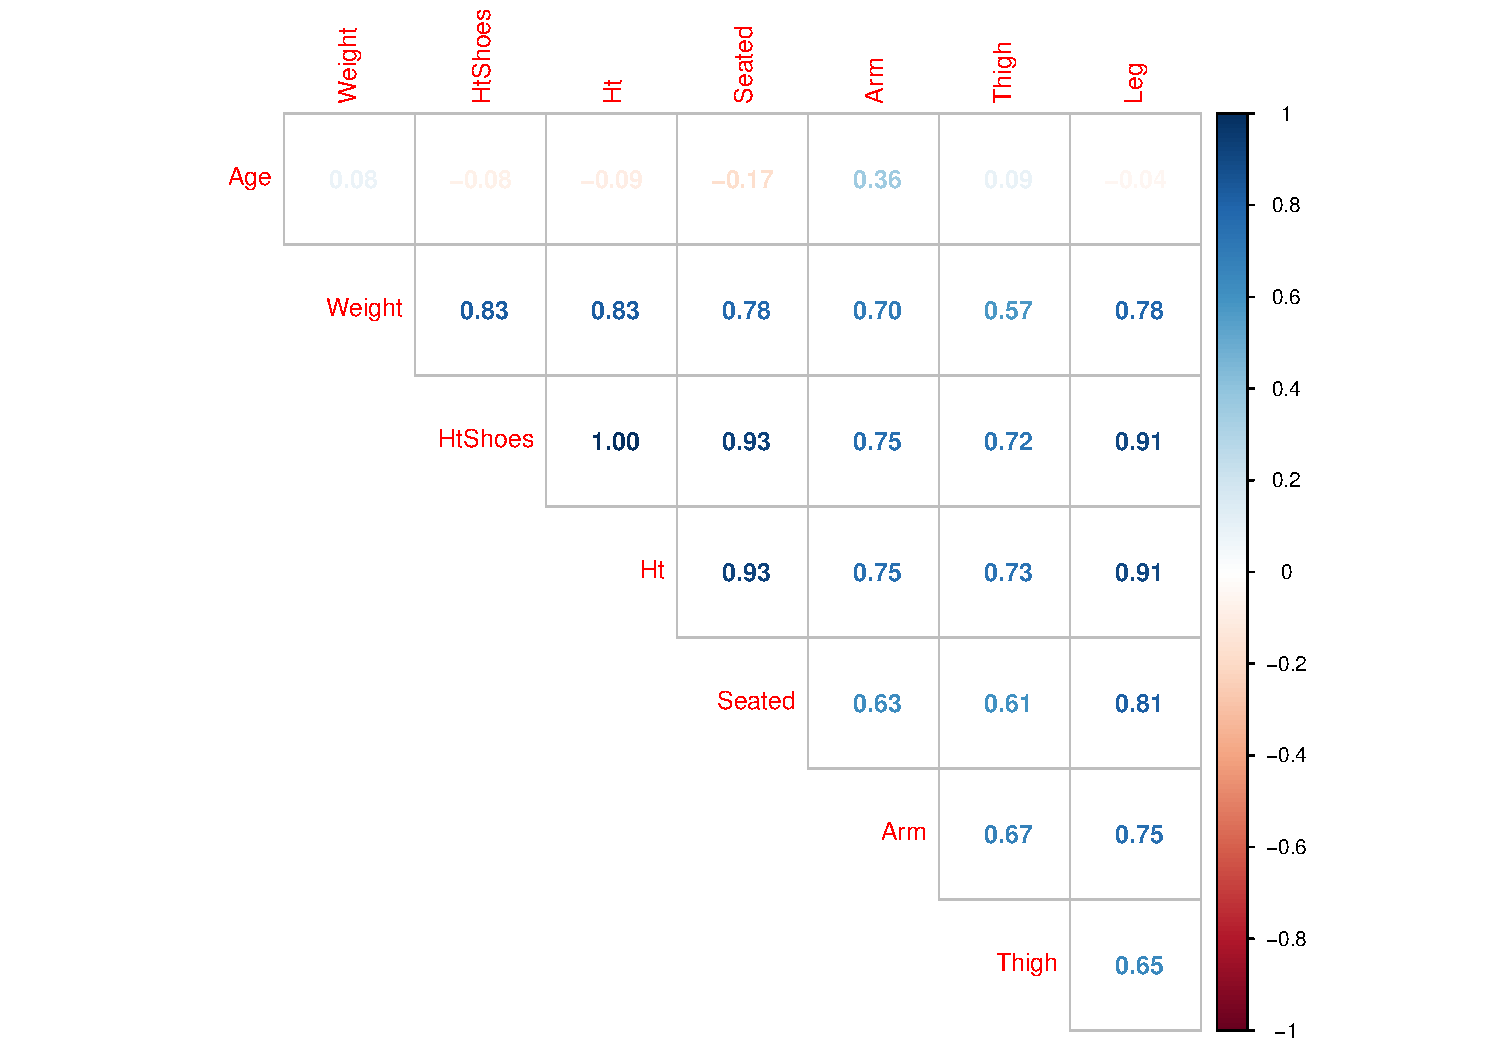
\includegraphics{2_1_files/figure-beamer/unnamed-chunk-12-1.pdf}
\end{frame}

\begin{frame}{Some Observations}
\protect\hypertarget{some-observations}{}
\begin{itemize}
\item
  Ht and HtShoes are 100\% correlated. Thus we just need one of these
  variable to be in the model
\item
  Ht and HtShoes are also very highly correlated to other predictors.
\end{itemize}
\end{frame}

\begin{frame}{}
\protect\hypertarget{section-9}{}
\begin{itemize}
\tightlist
\item
  Let's build a linear model among the predictors where HtShoes is the
  response.
\end{itemize}

\begin{table}[!h]
\centering
\begin{tabular}{lr}
\toprule
\cellcolor{gray!6}{F(7,30)} & \cellcolor{gray!6}{1313.26876}\\
R² & 0.99675\\
\cellcolor{gray!6}{Adj. R²} & \cellcolor{gray!6}{0.99599}\\
\bottomrule
\end{tabular}
\end{table} \begin{table}[!h]
\centering
\begin{threeparttable}
\begin{tabular}{lrrrr}
\toprule
  & Est. & S.E. & t val. & p\\
\midrule
\cellcolor{gray!6}{(Intercept)} & \cellcolor{gray!6}{0.23145} & \cellcolor{gray!6}{3.11789} & \cellcolor{gray!6}{0.07423} & \cellcolor{gray!6}{0.94132}\\
Age & 0.01446 & 0.01034 & 1.39802 & 0.17236\\
\cellcolor{gray!6}{Weight} & \cellcolor{gray!6}{-0.00241} & \cellcolor{gray!6}{0.00618} & \cellcolor{gray!6}{-0.38923} & \cellcolor{gray!6}{0.69986}\\
Ht & 1.00157 & 0.05021 & 19.94931 & 0.00000\\
\cellcolor{gray!6}{Seated} & \cellcolor{gray!6}{0.04869} & \cellcolor{gray!6}{0.06986} & \cellcolor{gray!6}{0.69693} & \cellcolor{gray!6}{0.49121}\\
\addlinespace
Arm & -0.02216 & 0.07290 & -0.30392 & 0.76329\\
\cellcolor{gray!6}{Thigh} & \cellcolor{gray!6}{-0.06058} & \cellcolor{gray!6}{0.04855} & \cellcolor{gray!6}{-1.24785} & \cellcolor{gray!6}{0.22174}\\
Leg & 0.01095 & 0.08822 & 0.12408 & 0.90208\\
\bottomrule
\end{tabular}
\begin{tablenotes}
\item Standard errors: OLS
\end{tablenotes}
\end{threeparttable}
\end{table}
\end{frame}

\begin{frame}{}
\protect\hypertarget{section-10}{}
\begin{itemize}
\item
  \(R^2 = 0.99675\) means that 99.675\% of variance of HtShoes are
  contained in the remaining predictors.
\item
  This means, there is only \(1-R^2 =\) 0.325\% of variance of HtShoes
  is unique to HtShoes.
\item
  Why we even need HtShoes in the model if it does not contribute much?
\end{itemize}
\end{frame}

\begin{frame}{}
\protect\hypertarget{section-11}{}
\begin{itemize}
\item
  \(1-R^2\) is called the tolerance of the variance.
\item
  The variance of Inflation Factor \(VIF = \frac{1}{1-R^2}\)
\item
  We want predictors have higher tolerance (more than .1) and lower VIF
  (smaller than 10)
\end{itemize}
\end{frame}

\begin{frame}{}
\protect\hypertarget{section-12}{}
\begin{table}[!h]
\centering
\begin{tabular}{lr}
\toprule
\cellcolor{gray!6}{F(7,30)} & \cellcolor{gray!6}{1313.27}\\
R² & 1.00\\
\cellcolor{gray!6}{Adj. R²} & \cellcolor{gray!6}{1.00}\\
\bottomrule
\end{tabular}
\end{table} \begin{table}[!h]
\centering
\begin{threeparttable}
\begin{tabular}{lrrrrr}
\toprule
  & Est. & S.E. & t val. & p & VIF\\
\midrule
\cellcolor{gray!6}{(Intercept)} & \cellcolor{gray!6}{0.23} & \cellcolor{gray!6}{3.12} & \cellcolor{gray!6}{0.07} & \cellcolor{gray!6}{0.94} & \cellcolor{gray!6}{NA}\\
Age & 0.01 & 0.01 & 1.40 & 0.17 & 1.88\\
\cellcolor{gray!6}{Weight} & \cellcolor{gray!6}{-0.00} & \cellcolor{gray!6}{0.01} & \cellcolor{gray!6}{-0.39} & \cellcolor{gray!6}{0.70} & \cellcolor{gray!6}{3.63}\\
Ht & 1.00 & 0.05 & 19.95 & 0.00 & 23.35\\
\cellcolor{gray!6}{Seated} & \cellcolor{gray!6}{0.05} & \cellcolor{gray!6}{0.07} & \cellcolor{gray!6}{0.70} & \cellcolor{gray!6}{0.49} & \cellcolor{gray!6}{8.81}\\
\addlinespace
Arm & -0.02 & 0.07 & -0.30 & 0.76 & 4.48\\
\cellcolor{gray!6}{Thigh} & \cellcolor{gray!6}{-0.06} & \cellcolor{gray!6}{0.05} & \cellcolor{gray!6}{-1.25} & \cellcolor{gray!6}{0.22} & \cellcolor{gray!6}{2.63}\\
Leg & 0.01 & 0.09 & 0.12 & 0.90 & 6.69\\
\bottomrule
\end{tabular}
\begin{tablenotes}
\item Standard errors: OLS
\end{tablenotes}
\end{threeparttable}
\end{table}
\end{frame}

\begin{frame}{Another Example}
\protect\hypertarget{another-example}{}
\begin{table}
\centering
\begin{tabular}[t]{r|r|r}
\hline
biking & smoking & heart\_disease\\
\hline
30.801246 & 10.8966080 & 11.7694228\\
\hline
65.129215 & 2.2195632 & 2.8540815\\
\hline
1.959664 & 17.5883305 & 17.1778035\\
\hline
44.800196 & 2.8025589 & 6.8166469\\
\hline
69.428454 & 15.9745046 & 4.0622235\\
\hline
54.403626 & 29.3331755 & 9.5500460\\
\hline
49.056162 & 9.0608458 & 7.6245070\\
\hline
4.784604 & 12.8350208 & 15.8546544\\
\hline
65.730788 & 11.9912973 & 3.0674617\\
\hline
35.257449 & 23.2776834 & 12.0984844\\
\hline
51.825567 & 14.4351184 & 6.4302482\\
\hline
52.936197 & 25.0748686 & 8.6082721\\
\hline
48.767479 & 11.0232710 & 6.7225238\\
\hline
26.166801 & 6.6457495 & 10.5978071\\
\hline
10.553075 & 5.9905063 & 14.0794783\\
\hline
47.163716 & 14.0978372 & 8.7448453\\
\hline
61.685256 & 16.8408167 & 5.4433420\\
\hline
33.944394 & 5.7585952 & 9.1623064\\
\hline
39.697624 & 12.6628694 & 9.7471858\\
\hline
63.124698 & 22.9174800 & 5.8582779\\
\hline
28.510129 & 14.8551064 & 11.7247416\\
\hline
18.525973 & 26.4049774 & 16.0281877\\
\hline
24.479470 & 26.9249607 & 15.0007154\\
\hline
18.358646 & 23.4319568 & 16.4882059\\
\hline
30.388184 & 16.9860864 & 12.3566075\\
\hline
52.985220 & 27.6890270 & 9.0884449\\
\hline
60.509448 & 3.9819621 & 3.2172143\\
\hline
45.247110 & 2.1374753 & 6.5937191\\
\hline
48.597044 & 10.3884264 & 6.6594202\\
\hline
25.139771 & 5.8363728 & 11.4829371\\
\hline
44.173095 & 3.9676057 & 7.9822275\\
\hline
61.146946 & 27.7834060 & 7.7224625\\
\hline
27.267898 & 16.8532932 & 12.1648167\\
\hline
49.527100 & 15.2497308 & 8.0274043\\
\hline
20.197206 & 10.3314895 & 13.4165474\\
\hline
18.811228 & 16.7534420 & 15.0873602\\
\hline
67.350765 & 23.8737268 & 5.2798634\\
\hline
29.904475 & 24.5845499 & 13.5076192\\
\hline
14.011760 & 21.0121418 & 15.9929864\\
\hline
45.815488 & 4.7161269 & 7.0406211\\
\hline
31.477251 & 22.1658255 & 13.2385262\\
\hline
17.108204 & 1.3528783 & 11.5357354\\
\hline
9.665083 & 3.5042963 & 12.8868168\\
\hline
23.933005 & 4.1858692 & 10.8944571\\
\hline
22.636301 & 13.6789828 & 13.4660327\\
\hline
27.247477 & 13.3797768 & 12.3288989\\
\hline
20.789602 & 19.4554286 & 14.4157831\\
\hline
46.613715 & 9.2493326 & 6.8093546\\
\hline
28.622632 & 12.4827339 & 11.3683650\\
\hline
21.127498 & 18.9413483 & 14.8253624\\
\hline
68.574348 & 1.8047036 & 0.6839264\\
\hline
41.684367 & 13.0672050 & 9.0888493\\
\hline
69.879593 & 17.3516599 & 4.2564834\\
\hline
9.817277 & 23.8189949 & 17.8341328\\
\hline
4.379280 & 20.6629714 & 17.4118109\\
\hline
28.610378 & 1.1479621 & 10.0558055\\
\hline
21.460016 & 22.9760018 & 15.0086341\\
\hline
27.601656 & 4.3883804 & 10.8936853\\
\hline
57.230504 & 12.8049999 & 5.3068180\\
\hline
26.397282 & 7.7639305 & 11.0243252\\
\hline
39.010480 & 0.7676801 & 8.7639297\\
\hline
11.527487 & 6.7396220 & 14.6003016\\
\hline
17.684287 & 8.2780091 & 13.8021255\\
\hline
19.935253 & 6.0764383 & 11.6320723\\
\hline
42.310040 & 8.4123966 & 7.4630017\\
\hline
1.119154 & 19.5503583 & 17.7101910\\
\hline
23.276822 & 14.3066349 & 13.2663850\\
\hline
14.965816 & 12.8691532 & 15.3003824\\
\hline
30.663350 & 16.6632038 & 11.7531562\\
\hline
22.925183 & 24.5987872 & 16.1991180\\
\hline
59.770308 & 8.7007692 & 5.6856819\\
\hline
70.456061 & 12.7407109 & 2.9059872\\
\hline
21.750385 & 18.8575107 & 14.1798442\\
\hline
49.360686 & 23.2094802 & 9.4660260\\
\hline
4.487242 & 23.4190000 & 18.7669334\\
\hline
14.693269 & 17.8743936 & 16.3479313\\
\hline
40.611628 & 25.9937106 & 12.0466432\\
\hline
8.764197 & 3.8990404 & 13.3730055\\
\hline
56.725412 & 16.1809774 & 6.7357709\\
\hline
60.551149 & 18.0652019 & 6.5167036\\
\hline
64.384893 & 10.5295310 & 4.5668945\\
\hline
20.262798 & 11.1787830 & 12.3790734\\
\hline
30.520086 & 12.4334774 & 11.1407355\\
\hline
30.461543 & 29.8608106 & 14.3299759\\
\hline
3.705894 & 21.4941886 & 17.8776920\\
\hline
15.082469 & 16.6152001 & 14.9359168\\
\hline
30.997842 & 29.0164264 & 13.7579867\\
\hline
14.625411 & 6.7983462 & 14.4789601\\
\hline
28.103061 & 14.7313505 & 12.7945549\\
\hline
34.680241 & 8.6381050 & 8.3317181\\
\hline
6.947463 & 26.1056583 & 18.6897979\\
\hline
26.860662 & 16.7194132 & 13.4876889\\
\hline
41.019323 & 12.9991873 & 10.2648899\\
\hline
31.932738 & 28.1828730 & 13.1737410\\
\hline
69.877147 & 26.3311967 & 6.0724855\\
\hline
63.029854 & 22.2471320 & 6.3567192\\
\hline
21.349999 & 12.8558535 & 13.7996830\\
\hline
3.811338 & 17.7237882 & 18.4623513\\
\hline
67.514106 & 26.9553999 & 6.5826851\\
\hline
12.580893 & 16.9897825 & 14.8556848\\
\hline
61.232197 & 4.6135505 & 4.3616062\\
\hline
64.332304 & 29.4237378 & 7.7073976\\
\hline
31.872439 & 16.2418978 & 10.5260293\\
\hline
11.936562 & 3.4865672 & 14.3914484\\
\hline
52.360268 & 19.8410769 & 7.8163886\\
\hline
22.516638 & 7.6951729 & 11.6647648\\
\hline
49.764822 & 3.5729441 & 6.2645744\\
\hline
22.792636 & 9.8168286 & 10.9117655\\
\hline
49.748748 & 20.4918307 & 8.7001979\\
\hline
68.204122 & 2.1929445 & 1.9664482\\
\hline
15.185101 & 14.5203621 & 14.5878253\\
\hline
58.046901 & 15.7135850 & 6.5593358\\
\hline
69.499688 & 23.1678748 & 5.7536536\\
\hline
2.616134 & 4.3190804 & 14.8517766\\
\hline
2.136343 & 25.8401303 & 19.2426878\\
\hline
25.771570 & 28.5403473 & 14.4293485\\
\hline
11.615646 & 6.3455289 & 14.4114830\\
\hline
17.197456 & 20.7334559 & 15.1981843\\
\hline
27.681662 & 18.6370085 & 11.5075952\\
\hline
9.648096 & 8.3700383 & 15.5763683\\
\hline
65.621956 & 14.1066235 & 4.0442469\\
\hline
46.556228 & 26.8937498 & 10.5427902\\
\hline
48.300472 & 12.0117869 & 7.2992774\\
\hline
15.141292 & 7.8937497 & 13.6191300\\
\hline
71.579351 & 18.9378855 & 4.0907648\\
\hline
4.681250 & 10.9882819 & 15.8685828\\
\hline
22.476723 & 25.9723233 & 14.8303440\\
\hline
49.296200 & 5.0887881 & 6.0737923\\
\hline
17.648135 & 27.1925636 & 15.1389680\\
\hline
9.413778 & 8.6085378 & 13.5250712\\
\hline
64.915668 & 10.8893906 & 3.7743880\\
\hline
3.950367 & 6.3595796 & 14.6357693\\
\hline
67.342457 & 16.6226193 & 3.7444984\\
\hline
71.238955 & 25.1941518 & 6.0015227\\
\hline
70.323878 & 26.2334743 & 5.2357312\\
\hline
28.424901 & 20.2084486 & 13.0038423\\
\hline
73.713732 & 14.1016522 & 2.9890677\\
\hline
56.058032 & 8.2061159 & 5.5239310\\
\hline
21.588199 & 2.5734949 & 11.3742898\\
\hline
16.276161 & 3.4634491 & 13.5987547\\
\hline
26.988690 & 15.8833260 & 12.9216726\\
\hline
11.326814 & 9.2306549 & 14.5243489\\
\hline
55.580584 & 7.6713074 & 5.7268270\\
\hline
50.603802 & 28.9184712 & 10.6355905\\
\hline
60.401739 & 24.8321410 & 7.5726142\\
\hline
71.486751 & 21.6373684 & 3.6684273\\
\hline
37.978507 & 13.9453443 & 10.1067938\\
\hline
48.692115 & 23.5640881 & 9.5990941\\
\hline
40.016400 & 7.8116349 & 7.6581870\\
\hline
32.148553 & 0.9690843 & 8.8739847\\
\hline
12.318283 & 26.8908058 & 17.7585948\\
\hline
31.659667 & 21.3995087 & 12.0931244\\
\hline
55.841893 & 2.2487162 & 4.5002273\\
\hline
28.826953 & 11.4098666 & 12.8126371\\
\hline
55.472287 & 5.2674378 & 4.9163834\\
\hline
54.354034 & 16.3415202 & 7.5917973\\
\hline
70.331699 & 15.0588637 & 3.0374318\\
\hline
54.062609 & 20.3888136 & 8.0511951\\
\hline
59.575645 & 24.7926381 & 8.5199279\\
\hline
2.818204 & 23.2461405 & 18.4829598\\
\hline
30.460335 & 2.5256544 & 8.9365829\\
\hline
22.343449 & 23.2046425 & 15.9085493\\
\hline
14.696886 & 9.8316822 & 13.2582035\\
\hline
70.902815 & 29.9140032 & 6.3350215\\
\hline
35.335113 & 9.1475020 & 9.7518942\\
\hline
72.173766 & 15.2736628 & 2.8283567\\
\hline
44.698217 & 10.0025889 & 7.4494126\\
\hline
70.361366 & 20.3399150 & 3.8971099\\
\hline
7.619084 & 26.6615229 & 18.6881304\\
\hline
29.673634 & 2.3967956 & 9.3879078\\
\hline
28.485683 & 12.6628036 & 11.2860570\\
\hline
67.423291 & 28.6574311 & 5.8094945\\
\hline
10.145069 & 11.3175196 & 14.8048065\\
\hline
59.989904 & 25.4558391 & 7.4743720\\
\hline
38.155015 & 20.1042221 & 11.5622808\\
\hline
15.466010 & 11.5711484 & 13.3774300\\
\hline
73.767713 & 16.1513316 & 2.3548085\\
\hline
31.179629 & 5.5684413 & 9.8617288\\
\hline
5.201611 & 4.3599032 & 15.6431142\\
\hline
50.249614 & 4.1290591 & 5.5419066\\
\hline
60.940141 & 21.8644959 & 5.4159174\\
\hline
20.068674 & 11.9294173 & 12.6884954\\
\hline
41.211215 & 4.1514402 & 7.5901660\\
\hline
72.394856 & 7.5198372 & 1.8701100\\
\hline
10.610969 & 19.3015155 & 16.7460356\\
\hline
45.579836 & 20.6168515 & 9.7984834\\
\hline
29.658506 & 12.1518990 & 12.8178071\\
\hline
40.056854 & 16.5064944 & 9.3926393\\
\hline
5.510300 & 17.8842193 & 16.0139209\\
\hline
32.056530 & 12.4794809 & 11.5360652\\
\hline
46.842870 & 27.3216486 & 10.2505847\\
\hline
42.425007 & 10.9547394 & 8.8282361\\
\hline
31.212374 & 7.7973828 & 9.7753859\\
\hline
13.176628 & 9.9874669 & 14.5477545\\
\hline
33.779739 & 0.9653903 & 6.9442975\\
\hline
70.690083 & 22.7107707 & 2.7084606\\
\hline
60.284951 & 15.1081402 & 4.9479908\\
\hline
16.003605 & 19.8941489 & 15.3662877\\
\hline
39.677219 & 10.2721672 & 9.5436557\\
\hline
12.885185 & 25.2101825 & 16.2725863\\
\hline
35.023451 & 22.6640373 & 12.5158362\\
\hline
10.343753 & 27.6468493 & 17.4485160\\
\hline
20.640892 & 15.3841384 & 14.5572879\\
\hline
63.238037 & 20.5047412 & 5.5609216\\
\hline
23.984565 & 7.6121169 & 11.5562573\\
\hline
44.014897 & 6.5796621 & 8.5037463\\
\hline
67.127924 & 5.8203635 & 2.5511506\\
\hline
36.538050 & 2.0528831 & 8.4950339\\
\hline
7.831481 & 26.8269709 & 17.5604514\\
\hline
40.395401 & 7.0274602 & 6.7390807\\
\hline
16.249914 & 28.3617369 & 17.3545771\\
\hline
47.584661 & 29.4683524 & 11.5999032\\
\hline
15.481362 & 18.8152012 & 14.9407560\\
\hline
70.085196 & 10.3826455 & 2.2392169\\
\hline
1.330485 & 28.7937440 & 20.4534962\\
\hline
61.542692 & 12.8374854 & 4.9734613\\
\hline
23.097771 & 0.9073611 & 10.6947889\\
\hline
65.069917 & 1.4876797 & 2.1856508\\
\hline
71.014542 & 15.2819055 & 4.0768235\\
\hline
64.065983 & 28.4724464 & 7.2862524\\
\hline
61.152760 & 2.1900536 & 3.5229763\\
\hline
22.672368 & 28.7353995 & 16.7786346\\
\hline
49.728740 & 3.4945424 & 5.0730746\\
\hline
35.480794 & 15.8501562 & 11.3729972\\
\hline
59.461885 & 18.8075341 & 5.6906489\\
\hline
31.697593 & 23.1906637 & 12.5378281\\
\hline
62.772108 & 15.2398176 & 4.9345783\\
\hline
58.668542 & 19.5857407 & 6.6620753\\
\hline
25.254140 & 7.1689519 & 12.0465147\\
\hline
22.722701 & 8.2882507 & 11.2963162\\
\hline
1.616922 & 1.4584368 & 16.3351186\\
\hline
10.353648 & 16.0131718 & 14.0886540\\
\hline
44.721586 & 7.2730788 & 7.6450248\\
\hline
29.224098 & 27.3570273 & 13.6443726\\
\hline
66.111593 & 18.6293941 & 4.5900481\\
\hline
46.728488 & 8.4995461 & 7.8255359\\
\hline
39.172427 & 17.5563764 & 10.7150869\\
\hline
9.937617 & 22.3426030 & 16.3846780\\
\hline
61.393845 & 22.9195492 & 6.8381847\\
\hline
21.608228 & 9.3488357 & 13.9959895\\
\hline
6.283610 & 20.1753292 & 17.5981661\\
\hline
61.436136 & 24.4659138 & 7.6206629\\
\hline
1.257841 & 15.1309519 & 16.7368633\\
\hline
4.699863 & 9.8599366 & 15.5694794\\
\hline
54.938223 & 13.0462165 & 6.2944988\\
\hline
7.749030 & 8.3870192 & 13.2815287\\
\hline
49.563424 & 16.2590213 & 8.1434851\\
\hline
29.731403 & 23.3339016 & 12.9964758\\
\hline
45.716267 & 23.8302604 & 9.2300743\\
\hline
47.537320 & 20.0742953 & 8.9378932\\
\hline
35.726016 & 8.9157682 & 10.5460251\\
\hline
35.912251 & 18.5148365 & 11.4380100\\
\hline
26.919990 & 11.5309853 & 12.1611678\\
\hline
34.162508 & 24.4145881 & 13.2060430\\
\hline
51.900538 & 27.3240290 & 9.5946227\\
\hline
73.143146 & 11.2752757 & 1.6857227\\
\hline
52.550886 & 13.8796797 & 7.4925558\\
\hline
10.664014 & 16.4896077 & 15.4418923\\
\hline
34.634851 & 4.9226945 & 8.8961039\\
\hline
37.693189 & 26.2662579 & 11.1773178\\
\hline
72.421679 & 4.2488265 & 0.7121819\\
\hline
30.161485 & 6.6110456 & 9.8354744\\
\hline
67.121405 & 8.4784824 & 3.1181517\\
\hline
10.262000 & 26.8565236 & 17.1060395\\
\hline
17.525751 & 4.7638941 & 11.9488893\\
\hline
66.840014 & 0.5258500 & 0.9875364\\
\hline
70.299739 & 6.4237343 & 1.1048204\\
\hline
34.229590 & 17.7648414 & 11.2714178\\
\hline
42.594866 & 26.2857438 & 11.6009394\\
\hline
73.987237 & 16.9157391 & 3.8353451\\
\hline
69.310829 & 4.6557367 & 2.2016530\\
\hline
38.636658 & 18.2480098 & 9.5133839\\
\hline
24.699356 & 4.6039660 & 12.1074100\\
\hline
55.370253 & 17.2038510 & 7.2310693\\
\hline
32.170214 & 5.0175149 & 9.9049713\\
\hline
67.779633 & 15.1993371 & 4.6800975\\
\hline
16.057724 & 19.1118900 & 14.6563521\\
\hline
39.333217 & 15.1034692 & 9.3244739\\
\hline
37.665190 & 24.9718414 & 11.1056306\\
\hline
28.480246 & 17.3199216 & 11.7295703\\
\hline
73.932909 & 26.5264341 & 5.3340374\\
\hline
61.313971 & 16.8076136 & 4.8419280\\
\hline
67.822195 & 26.8826561 & 6.2617038\\
\hline
1.466301 & 28.2069104 & 20.1852906\\
\hline
61.925511 & 26.3258096 & 6.8571743\\
\hline
25.665004 & 23.2615382 & 13.6432671\\
\hline
36.237608 & 20.9340928 & 12.7512095\\
\hline
45.457607 & 25.7596081 & 10.8655224\\
\hline
49.022959 & 3.2280954 & 5.8429680\\
\hline
63.799428 & 29.1247242 & 7.6188035\\
\hline
4.470326 & 4.3553675 & 13.7798360\\
\hline
47.695866 & 28.3878511 & 10.1749400\\
\hline
4.341424 & 8.0329811 & 15.1727164\\
\hline
66.971620 & 24.2198387 & 5.7955982\\
\hline
34.032646 & 13.0622367 & 10.3819438\\
\hline
13.625346 & 1.4167141 & 11.8208854\\
\hline
54.821433 & 10.6239231 & 6.2237844\\
\hline
18.205567 & 15.9476017 & 13.9029794\\
\hline
51.692701 & 19.1996174 & 6.9520550\\
\hline
7.480637 & 19.4392335 & 16.6418807\\
\hline
47.355227 & 15.3457820 & 9.0957486\\
\hline
38.204290 & 23.5397917 & 11.7785962\\
\hline
33.742643 & 14.0819166 & 10.2335875\\
\hline
40.555015 & 2.7828646 & 6.5730508\\
\hline
70.208596 & 13.7516893 & 5.3190941\\
\hline
26.155009 & 7.4422319 & 12.3513903\\
\hline
17.751723 & 3.4824026 & 11.4296860\\
\hline
71.847044 & 13.0407691 & 2.0628619\\
\hline
60.021979 & 4.2868104 & 4.1138786\\
\hline
60.270390 & 8.7861543 & 4.5911728\\
\hline
33.922205 & 24.3928492 & 11.3852091\\
\hline
43.300519 & 8.2850748 & 6.5585796\\
\hline
22.891589 & 2.4011628 & 10.9717609\\
\hline
57.095671 & 3.2911638 & 4.6269659\\
\hline
40.124049 & 13.9695702 & 9.9049209\\
\hline
37.332538 & 12.7516464 & 10.7042342\\
\hline
32.634373 & 13.7179209 & 10.3775691\\
\hline
43.909341 & 26.0620820 & 11.4335113\\
\hline
15.489999 & 19.5430617 & 15.2399655\\
\hline
52.034081 & 16.2070389 & 8.2689831\\
\hline
3.960526 & 27.4715448 & 19.4319601\\
\hline
61.303891 & 15.4111217 & 5.4789087\\
\hline
56.367512 & 17.5203572 & 6.8083997\\
\hline
34.530051 & 16.7816632 & 10.7291815\\
\hline
70.950558 & 3.5211730 & 0.7049961\\
\hline
44.572770 & 17.1550494 & 8.3108977\\
\hline
9.816417 & 18.0027014 & 16.7913828\\
\hline
14.242695 & 26.7242731 & 17.3705338\\
\hline
15.137385 & 3.2812824 & 12.7344968\\
\hline
39.905489 & 19.7205943 & 8.8858633\\
\hline
13.730690 & 14.2177350 & 14.2983625\\
\hline
51.563683 & 23.3450455 & 8.5490950\\
\hline
74.011080 & 18.8543469 & 3.2962178\\
\hline
13.939865 & 27.2540442 & 15.9893714\\
\hline
36.374862 & 25.3954955 & 11.6298290\\
\hline
14.732989 & 19.4709192 & 14.4080750\\
\hline
6.178654 & 15.5468701 & 15.9778522\\
\hline
8.128956 & 5.8893583 & 14.4437737\\
\hline
9.727759 & 15.2972538 & 15.5885430\\
\hline
20.226774 & 28.1769618 & 16.5178715\\
\hline
46.020846 & 18.0521329 & 9.2319707\\
\hline
33.284619 & 17.3050400 & 11.2694843\\
\hline
19.909001 & 19.0605707 & 14.4660128\\
\hline
8.633643 & 4.3829289 & 14.4858121\\
\hline
50.898031 & 29.8252593 & 10.8115183\\
\hline
1.576452 & 9.0612731 & 14.4343940\\
\hline
10.389193 & 23.6915084 & 16.9616280\\
\hline
28.896313 & 24.2375831 & 13.7241183\\
\hline
68.029425 & 13.2735594 & 4.0660948\\
\hline
5.471788 & 16.0808894 & 17.6180620\\
\hline
48.777851 & 27.7454919 & 8.9976366\\
\hline
61.356691 & 17.9649971 & 4.9460902\\
\hline
64.173931 & 19.0373520 & 6.0609886\\
\hline
2.977160 & 3.8397647 & 15.1627752\\
\hline
69.992342 & 20.2625714 & 3.6893645\\
\hline
65.963766 & 3.5069213 & 2.7186641\\
\hline
19.374553 & 6.1153180 & 11.5437192\\
\hline
57.995069 & 16.3960303 & 5.7177334\\
\hline
9.661735 & 4.3501964 & 13.6273518\\
\hline
24.953993 & 23.2441339 & 13.6705821\\
\hline
62.061053 & 21.2032056 & 6.7150779\\
\hline
49.888796 & 3.8610316 & 5.3261272\\
\hline
69.776191 & 20.2866413 & 4.5242760\\
\hline
29.578742 & 18.7836006 & 11.8311383\\
\hline
59.869018 & 22.8854866 & 7.3223322\\
\hline
19.071488 & 27.0881800 & 16.6098257\\
\hline
20.803894 & 5.2645876 & 11.0583055\\
\hline
2.633935 & 18.3404030 & 16.3756622\\
\hline
39.944085 & 14.5277596 & 10.0490669\\
\hline
48.547680 & 5.0688691 & 6.5079475\\
\hline
26.332030 & 26.6869350 & 15.1165636\\
\hline
15.347194 & 22.4262563 & 17.2692334\\
\hline
74.583779 & 16.1937408 & 2.9116599\\
\hline
61.534993 & 17.0459635 & 5.9054458\\
\hline
19.651335 & 1.3962618 & 11.7697859\\
\hline
23.315546 & 20.6625244 & 13.7515775\\
\hline
14.700212 & 28.3058238 & 17.0171583\\
\hline
13.377701 & 29.6848022 & 17.2139369\\
\hline
32.484626 & 25.2504638 & 13.1917033\\
\hline
39.246899 & 15.3416817 & 10.3885655\\
\hline
8.522310 & 29.9467431 & 17.8578487\\
\hline
37.177186 & 22.3559719 & 10.5036890\\
\hline
70.700683 & 19.0571762 & 2.8284841\\
\hline
68.212733 & 15.3178344 & 4.4809930\\
\hline
31.714463 & 28.7458214 & 13.0160451\\
\hline
65.201713 & 24.2065845 & 7.1849464\\
\hline
64.376918 & 29.2571132 & 7.3303757\\
\hline
67.256755 & 15.0187118 & 4.6315166\\
\hline
21.537676 & 4.7600703 & 10.3661423\\
\hline
63.596727 & 12.5153904 & 3.4530267\\
\hline
39.993010 & 14.5087353 & 9.5094184\\
\hline
70.578968 & 11.2198596 & 2.6547061\\
\hline
54.101324 & 25.9821230 & 8.8541074\\
\hline
22.358288 & 21.6506575 & 15.0308207\\
\hline
60.584615 & 6.4720628 & 3.3491379\\
\hline
61.296241 & 4.2479007 & 3.3978433\\
\hline
41.443284 & 5.1569665 & 7.1491787\\
\hline
58.430433 & 0.7342280 & 3.2338332\\
\hline
71.670317 & 0.9415583 & 0.5546971\\
\hline
61.008149 & 7.6460379 & 3.5986787\\
\hline
69.671782 & 24.9687638 & 5.8505170\\
\hline
19.313206 & 29.6571442 & 16.2651030\\
\hline
38.166866 & 4.2476656 & 7.2579462\\
\hline
24.760319 & 6.5129285 & 11.5776716\\
\hline
12.949559 & 27.0340559 & 18.6396922\\
\hline
17.966363 & 26.8311231 & 16.1647940\\
\hline
4.158496 & 19.6597161 & 17.0589359\\
\hline
50.837966 & 20.0001457 & 7.9306012\\
\hline
8.796572 & 16.5032820 & 16.5272933\\
\hline
27.423996 & 18.2377258 & 11.5944099\\
\hline
5.782733 & 6.8057129 & 15.8369336\\
\hline
4.445668 & 27.3295368 & 18.6734573\\
\hline
30.120726 & 29.3418945 & 14.9898130\\
\hline
29.047919 & 29.2027903 & 13.7702316\\
\hline
26.723292 & 11.5928445 & 11.4241149\\
\hline
38.116560 & 17.0259702 & 8.3455735\\
\hline
45.859855 & 2.6209658 & 5.8095431\\
\hline
62.021049 & 23.8830499 & 6.9595020\\
\hline
6.057336 & 14.2552872 & 17.1337446\\
\hline
4.731341 & 24.1359724 & 19.5817260\\
\hline
25.767233 & 19.8270986 & 13.1750007\\
\hline
25.906997 & 16.1600287 & 13.6480773\\
\hline
71.930577 & 19.4163691 & 4.1132188\\
\hline
57.978406 & 20.5598091 & 7.5006118\\
\hline
21.822555 & 15.5006589 & 13.3798074\\
\hline
15.371938 & 23.4066160 & 14.0716450\\
\hline
67.471759 & 14.6354724 & 4.6955205\\
\hline
64.485419 & 5.8788732 & 2.9787686\\
\hline
35.736667 & 9.3960224 & 9.5718912\\
\hline
6.324214 & 5.2075066 & 14.8081496\\
\hline
64.033751 & 29.5593251 & 8.5705833\\
\hline
66.015502 & 13.5683691 & 4.1847701\\
\hline
3.220291 & 9.1764671 & 16.4996389\\
\hline
36.328194 & 8.2483419 & 9.7801651\\
\hline
29.866577 & 2.3942733 & 9.4468988\\
\hline
57.475925 & 15.7790716 & 6.0360129\\
\hline
18.126784 & 10.7587843 & 13.3344281\\
\hline
31.847309 & 22.1871573 & 13.2836703\\
\hline
63.753105 & 9.9062485 & 3.4020804\\
\hline
30.519444 & 18.1421048 & 11.6585708\\
\hline
74.205816 & 9.2990963 & 1.5734290\\
\hline
33.020247 & 0.6817504 & 8.5578541\\
\hline
22.530761 & 16.3310107 & 13.7196390\\
\hline
2.010308 & 1.7517191 & 14.0074901\\
\hline
11.099022 & 17.5277122 & 14.8979609\\
\hline
25.301649 & 18.1137812 & 13.1931753\\
\hline
33.157137 & 17.5565040 & 12.0628147\\
\hline
28.569941 & 15.9952260 & 12.0749260\\
\hline
60.031747 & 11.3688387 & 5.0722812\\
\hline
18.951146 & 13.9546247 & 13.4705063\\
\hline
24.727982 & 25.6012842 & 13.7237396\\
\hline
74.907111 & 5.6959430 & 1.0944887\\
\hline
10.530125 & 14.9603882 & 15.5819986\\
\hline
74.210494 & 22.5850200 & 4.2963770\\
\hline
36.290536 & 25.2679184 & 12.5665225\\
\hline
55.198777 & 15.3344487 & 7.0159902\\
\hline
57.044609 & 9.6842191 & 5.7281349\\
\hline
68.658906 & 22.4306836 & 5.3569752\\
\hline
40.317458 & 1.6025254 & 6.7852343\\
\hline
31.417332 & 8.1845130 & 9.7932399\\
\hline
71.440415 & 12.8449456 & 3.2634022\\
\hline
34.836579 & 29.8244807 & 13.3703392\\
\hline
39.349849 & 13.6011709 & 8.8679251\\
\hline
73.848167 & 0.6420440 & 0.5518982\\
\hline
40.764848 & 11.5974803 & 8.4629523\\
\hline
60.630416 & 23.7849810 & 5.9764276\\
\hline
74.508779 & 22.5206403 & 4.3031890\\
\hline
56.210806 & 19.2488506 & 6.5126756\\
\hline
11.658029 & 26.7341762 & 17.4739403\\
\hline
6.295051 & 19.4351915 & 17.7621148\\
\hline
60.587355 & 8.1735868 & 4.9380589\\
\hline
56.151543 & 28.3524443 & 10.1612021\\
\hline
74.221991 & 26.0782411 & 4.6313983\\
\hline
25.443047 & 13.2003989 & 12.3580352\\
\hline
36.368318 & 23.6979059 & 11.2829462\\
\hline
25.887693 & 8.1590235 & 10.8874134\\
\hline
59.350253 & 20.3678154 & 7.6653459\\
\hline
11.883447 & 1.1427967 & 12.7884505\\
\hline
4.817058 & 27.5778350 & 18.5036637\\
\hline
7.582143 & 29.6442147 & 18.0812684\\
\hline
54.181002 & 5.9596483 & 5.3516192\\
\hline
33.262015 & 6.8121297 & 10.3723287\\
\hline
36.086220 & 13.7865546 & 9.7315448\\
\hline
55.663943 & 14.9632192 & 6.9162586\\
\hline
22.719661 & 1.0247563 & 10.8938936\\
\hline
41.178991 & 7.5752679 & 7.8313847\\
\hline
22.021893 & 19.4992577 & 13.7706394\\
\hline
69.927963 & 25.9843899 & 6.7560155\\
\hline
41.642072 & 0.5330593 & 5.9256803\\
\hline
70.194411 & 16.2928029 & 4.7070094\\
\hline
50.831908 & 6.0260661 & 5.5854932\\
\hline
68.884065 & 10.5429959 & 3.1093377\\
\hline
21.599231 & 7.6043297 & 12.3736910\\
\hline
47.660440 & 27.5624638 & 11.2943916\\
\hline
45.097203 & 21.3856201 & 9.6167625\\
\hline
8.279743 & 6.4237195 & 13.4951677\\
\hline
42.345863 & 20.7413275 & 10.1158651\\
\hline
30.774254 & 23.6101750 & 11.8435558\\
\hline
\end{tabular}
\end{table}
\end{frame}

\begin{frame}{}
\protect\hypertarget{section-13}{}
\begin{table}[!h]
\centering
\begin{tabular}{lr}
\toprule
\cellcolor{gray!6}{Observations} & \cellcolor{gray!6}{498}\\
Dependent variable & heart\_disease\\
\cellcolor{gray!6}{Type} & \cellcolor{gray!6}{OLS linear regression}\\
\bottomrule
\end{tabular}
\end{table} \begin{table}[!h]
\centering
\begin{tabular}{lr}
\toprule
\cellcolor{gray!6}{F(2,495)} & \cellcolor{gray!6}{11895.24}\\
R² & 0.98\\
\cellcolor{gray!6}{Adj. R²} & \cellcolor{gray!6}{0.98}\\
\bottomrule
\end{tabular}
\end{table} \begin{table}[!h]
\centering
\begin{threeparttable}
\begin{tabular}{lrrrrr}
\toprule
  & Est. & S.E. & t val. & p & VIF\\
\midrule
\cellcolor{gray!6}{(Intercept)} & \cellcolor{gray!6}{14.98} & \cellcolor{gray!6}{0.08} & \cellcolor{gray!6}{186.99} & \cellcolor{gray!6}{0.00} & \cellcolor{gray!6}{NA}\\
biking & -0.20 & 0.00 & -146.53 & 0.00 & 1.00\\
\cellcolor{gray!6}{smoking} & \cellcolor{gray!6}{0.18} & \cellcolor{gray!6}{0.00} & \cellcolor{gray!6}{50.39} & \cellcolor{gray!6}{0.00} & \cellcolor{gray!6}{1.00}\\
\bottomrule
\end{tabular}
\begin{tablenotes}
\item Standard errors: OLS
\end{tablenotes}
\end{threeparttable}
\end{table}
\end{frame}

\begin{frame}{Creating multicolinearity}
\protect\hypertarget{creating-multicolinearity}{}
\begin{itemize}
\item
  We want to purposely create a new variable that colinear with the two
  original variables.
\item
  \(x3 = 3*biking - 10*smoking + \epsilon\), \(\epsilon \sim N(0,1)\)
\end{itemize}
\end{frame}

\begin{frame}{Creating multicolinearity}
\protect\hypertarget{creating-multicolinearity-1}{}
\begin{table}[!h]
\centering
\begin{tabular}{lr}
\toprule
\cellcolor{gray!6}{Observations} & \cellcolor{gray!6}{498}\\
Dependent variable & heart\_disease\\
\cellcolor{gray!6}{Type} & \cellcolor{gray!6}{OLS linear regression}\\
\bottomrule
\end{tabular}
\end{table} \begin{table}[!h]
\centering
\begin{tabular}{lr}
\toprule
\cellcolor{gray!6}{F(3,494)} & \cellcolor{gray!6}{7936.46}\\
R² & 0.98\\
\cellcolor{gray!6}{Adj. R²} & \cellcolor{gray!6}{0.98}\\
\bottomrule
\end{tabular}
\end{table} \begin{table}[!h]
\centering
\begin{threeparttable}
\begin{tabular}{lrrrrr}
\toprule
  & Est. & S.E. & t val. & p & VIF\\
\midrule
\cellcolor{gray!6}{(Intercept)} & \cellcolor{gray!6}{15.02} & \cellcolor{gray!6}{0.08} & \cellcolor{gray!6}{177.09} & \cellcolor{gray!6}{0.00} & \cellcolor{gray!6}{NA}\\
biking & -0.09 & 0.09 & -1.05 & 0.30 & 4387.17\\
\cellcolor{gray!6}{smoking} & \cellcolor{gray!6}{-0.17} & \cellcolor{gray!6}{0.30} & \cellcolor{gray!6}{-0.58} & \cellcolor{gray!6}{0.56} & \cellcolor{gray!6}{7255.38}\\
x3 & -0.04 & 0.03 & -1.17 & 0.24 & 11470.78\\
\bottomrule
\end{tabular}
\begin{tablenotes}
\item Standard errors: OLS
\end{tablenotes}
\end{threeparttable}
\end{table}
\end{frame}

\begin{frame}{What to do?}
\protect\hypertarget{what-to-do}{}
\begin{itemize}
\item
  If the main goal of building the model is for prediction, then we do
  not need to do anything. Multuiconolinearity does not affect the
  predictive power of the model.
\item
  Check if there is any duplicate predictor
\item
  Remove redundant variable
\item
  Use variable selections methods such as stepwise or LASSO
\item
  Use methods to create new set of variables from the original
  variables, such as principal component analysis.
\end{itemize}
\end{frame}



\end{document}
